\documentclass[11pt, spanish, a4paper, twoside]{article}

% Versión 1.er cuat 2021 Víctor Bettachini < vbettachini@unlam.edu.ar >

\usepackage[T1]{fontenc}
\usepackage[utf8]{inputenc}

\usepackage[spanish, es-tabla]{babel}
% \def\spanishoptions{argentina} % Was macht dass?
% \usepackage{babelbib}
% \selectbiblanguage{spanish}
% \addto\shorthandsspanish{\spanishdeactivate{~<>}}


\usepackage{graphicx}
\graphicspath{{./figuras/}{../LaTeX/}{../figurasLaTeX/}}
% \usepackage{float}

\usepackage[arrowdel]{physics}
\newcommand{\pvec}[1]{\vec{#1}\mkern2mu\vphantom{#1}}
% \usepackage{units}
\usepackage[separate-uncertainty= true, multi-part-units= single, range-units= single, range-phrase= {~a~}, locale= FR]{siunitx}
\usepackage{isotope} % $\isotope[A][Z]{X}\to\isotope[A-4][Z-2]{Y}+\isotope[4][2]{\alpha}

\usepackage{tasks}
\usepackage[inline]{enumitem}
% \usepackage{enumerate}

\usepackage{hyperref}

% \usepackage{amsmath}
% \usepackage{amstext}
% \usepackage{amssymb}

\usepackage{tikz}
\usepackage{tikz-3dplot}
\usepackage{tikz-dimline}
\usetikzlibrary{calc}
% \usetikzlibrary{math}
\usetikzlibrary{arrows.meta}
\usetikzlibrary{snakes}
\usetikzlibrary{decorations}
\usetikzlibrary{decorations.pathmorphing}
\usetikzlibrary{patterns}

\usepackage[hmargin=1cm,vmargin=3cm, top= 0.75cm,nohead]{geometry}

\usepackage{lastpage}
\usepackage{fancyhdr}
\pagestyle{fancyplain}
\fancyhf{}
\setlength\headheight{28.7pt} 
\fancyhead[LE, LO]{\textbf{Mecánica Analítica Computacional} }
% \fancyhead[LE, LO]{\textbf{Mecánica General} }
\fancyhead[RE, RO]{\href{https://ingenieria.unlam.edu.ar/}{$\vcenter{\hbox{
\includegraphics[height=1cm]{ambos.pdf}}}$}}
\fancyfoot{\href{https://creativecommons.org/licenses/by-nc-sa/4.0/deed.es_ES}{$\vcenter{\hbox{
\includegraphics[height=0.4cm]{by-nc-sa_80x15.pdf}}}$} \href{https://ingenieria.unlam.edu.ar/}{DIIT - UNLaM}}
\fancyfoot[C]{ {\tiny Actualizado al \today} }
\fancyfoot[RO, LE]{Pág. \thepage/\pageref{LastPage}}
\renewcommand{\headrulewidth}{0pt}
\renewcommand{\footrulewidth}{0pt}



\begin{document}

\begin{center}
  % \textsc{\large Mecánica general}\\
  \textsc{\large Coordenadas generalizadas | Ligaduras | Energía}
\end{center}
\noindent
Los problemas marcados con (*) tienen alguna dificultad adicional, no dude en consultar.

\begin{enumerate}

		%\item \begin{minipage}[t][7.1cm]{0.75\textwidth}
%\textbf{Péndulo simple} [Marion (e) ex. 7.2] \\
%Obtenga la ecuación diferencial que describe la dinámica de una pesa que ``pendulea'' en el extremo de una cuerda.
%\begin{enumerate}
%	\item Si el péndulo oscila dentro del plano \(\hat{x}, \hat{y}\).
%		¿En que sistema de coordenadas resolverá el problema? 
%		¿Cuál coordenada es relevante para describir la dinámica? 
%	\item Enumere las aproximaciones del modelo de péndulo que resolverá que lo diferencian de uno que puede armar en el laboratorio.
%	\item Calcule la energía potencial de la pesa en el campo gravitatorio.
%	¿Para qué sirve eso?
%	Las fuerzas que surgen de un campo son fácilmente calculables usando que \(\vec{F} = - \vec{\nabla} V\), es decir, \emph{la fuerza es igual al negativo del gradiente del potencial}.
%	\item Escriba la 2.a ley de Newton para la coordenada relevante.
%	\item Resuelva la ecuación de la dinámica y obtenga la frecuencia de oscilación.
%\end{enumerate}
%\end{minipage}
%\begin{minipage}[c][0cm][t]{0.2\textwidth}
%%	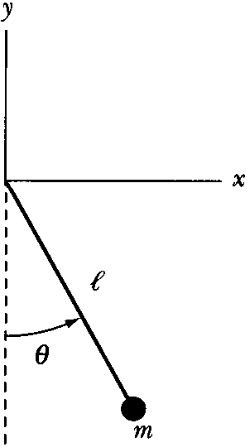
\includegraphics[width=\textwidth]{marion_fig7_1}
%%	\includegraphics[width=\textwidth]{\detokenize{pénduloHorizontal}}
%	\begin{tikzpicture}[scale= 1.0]
%	\draw [arrows=-latex] (-1,2) -> (-1,1) node [above=15, right=2] {\(\vec{g}\)}; % g vertical
%		\draw [ultra thick] (-1.5,3) -- (2,3);
%		\fill [pattern = north east lines] (-1.5,3) rectangle (2,3.2); % techo
%		\draw [dashed] (0,3) -- (0,-.25);	% vertical
%		\draw [thick] (0,3) -- +(-60:3) node[midway,above,right=2] {\(\ell\)};	% inclinada +:relativa, -60 grados, longitud 3
%		\shade [ball color=black!80] ($(0,3)+(-60:3)$) circle(0.25) node [] {\color{white} $m$};
%    \draw [arrows=-latex] (0,.4) -> (1.25,.4) node [midway, above] {\( \psi \)}; % desplazamiento horizontal
%		\draw [arrows=-latex] (0,0) arc [start angle=-90, end angle=-65, radius=3] node [below=12, left=8] {\( \varphi \)};
%	\end{tikzpicture}
%\end{minipage}
%%\vspace{-2.5cm}
%

%\subsection*{Fuerza como gradiente de un potencial}
%% Vizcaino carpeta
%\item Una partícula esta sometida a una fuerza \(\vec{F}(x)= \left( -k x + \frac{a}{x^3}\right) \hat{x}\)
%\begin{enumerate}
%    \item Hallar el potencial \(U(x)\) y graficarlo.
%    \item Discutir los tipos de movimientos posibles.
%    \item Determinar las posiciones de equilibrio estable y encuentre la solución general de la dinámica de la partícula, \(\vec{r}(t)\).
%    \item Interpretar el movimiento en el límite \(E^2 \gg k a\). ¿Cuanto vale el periodo de las oscilaciones?
%    \item Ídem. anterior en el límite \(E^2 \rightarrow k a\) con \(E^2 > k a\).
%\end{enumerate}



%\item \begin{minipage}[t][3cm]{0.7\textwidth}
%\textbf{Péndulo ideal rígido} [Marion ex. 7.2]\\
%Escriba y resuelva la ecuación que describe la dinámica de un péndulo de longitud $\ell$ en presencia de un campo gravitatorio de constante $g$. Discuta todas las aproximaciones que realiza.
%\end{minipage}
%\begin{minipage}[c][1cm][t]{0.25\textwidth}
%%	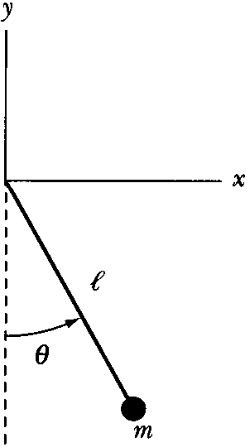
\includegraphics[width=0.75\textwidth]{marion_fig7_1}
%%	\includegraphics[width=\textwidth]{\detokenize{pénduloHorizontal}}
%	\begin{tikzpicture}
%	%\begin{tikzpicture}[scale= 1.2]
%  	\draw [arrows=- triangle 45] (-1,2) -> (-1,1) node [above=15, right=2] {\(\vec{g}\)}; % g vertical
%		\draw [ultra thick] (-1.5,3) -- (2.5,3);
%		\fill [pattern = north east lines] (-1.5,3) rectangle (2.5,3.2); % techo
%		\draw [dashed] (0,3) -- (0,0);	% vertical
%		\draw [thick] (0,3) -- +(-60:3) node[midway,above,right=2] {\(\ell\)};	% inclinada +:relativa, -60 grados, longitud 3
%		% \draw [thick] (0,3) -- +(-60:3) node[midway,above,sloped] {\(l\)};	% inclinada +:relativa, -60 grados, longitud 3
%    \fill (0,3)+(-60:3) circle [radius=0.25] node [text=white] { \( \mathrm{m} \) }; % masa izq
%    \draw [thin, arrows=- triangle 45] (0,.4) -> (1.25,.4) node [midway, above] {\( \psi \)}; % desplazamiento horizontal
%    % \draw [thin, arrows=- triangle 45] (0,.4) -> (1.25,.4) node [above=8, left=8] {\( \psi \)}; % desplazamiento horizontal
%		\draw [thin, arrows=- triangle 45] (0,0) arc [start angle=-90, end angle=-65, radius=3] node [below=12, left=8] {\( \varphi \)};
%	\end{tikzpicture}
%\end{minipage}




\item
	\begin{minipage}[t][5cm]{0.7\textwidth}
		\textbf{Péndulo con punto de suspensión libre} [Landau \S5 ej. 2]\\
		La partícula de masa \(m_2\) pende de una barra rígida de longitud \(\ell\) de masa despreciable.
		El otro extremo de la misma está engarzada a una barra rígido horizontal dispuesta a lo largo del eje \(\hat{x}\).
		El dispositivo de engarze tiene una masa \(m_1\).
		\begin{enumerate}
			\item Escriba la energía cinética, \(T\) y potencial, \(V\), en función de las coordenadas generalizadas sugeridas por las figura.
			\item Verifique que al fijar la masa \(m_1\) recupera las expresiones de \(T\) y \(V\) de un péndulo ideal.
		\end{enumerate}
	\end{minipage}
	\begin{minipage}[c][1cm][t]{0.3\textwidth}
		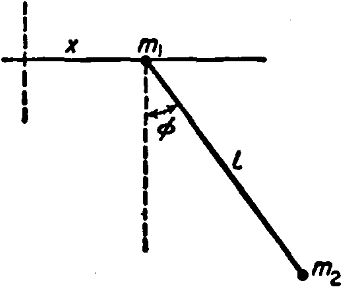
\includegraphics[width=0.75\textwidth]{landauS52_fig2.png}
	\end{minipage}



\item
	\begin{minipage}[t][4cm]{0.7\textwidth}
		\textbf{Péndulo doble} [Landau \S5 ej. 1]\\
		Una barra rígida de longitud \(\ell_1\) tiene una masa despreciable respecto a la de la partícula de masa \(m_1\) fija a su extremo.
		A su vez de esta última pende otra barra rígida, de longitud \(\ell_2\) que en su extremo tiene otra partícula de masa \(m_2\), también mucho mayor que aquella de la barra.
		\begin{enumerate}
			\item Calcule la energía cinética, \(T\) y potencial, \(V\).
			\item Verifique que recupera \(T\) y \(V\) de un péndulo simple de asumir \(m_1=0\), \(\varphi_1 = \varphi_2 = \varphi\) y \(\ell_1 = \ell_2 = \frac{l}{2}\).
		\end{enumerate}
		% Ayuda: \( \cos(\alpha \pm \beta) = \cos{ \alpha} \cos{ \beta \mp \sin \alpha} \sin{ \beta } \)
	\end{minipage}
	\begin{minipage}[c][0.5cm][t]{0.3\textwidth}
		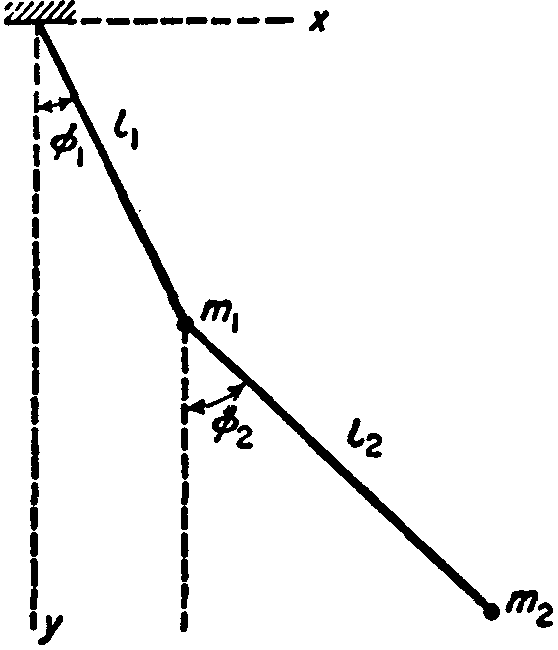
\includegraphics[width=0.75\textwidth]{landauS52_fig1.png}
	\end{minipage}



\item
	\begin{minipage}[t][7.1cm]{0.5\textwidth}
		(*) \textbf{Péndulo con punto de suspensión en rotación} [Marion (e) ex. 7.5] [Landau \S5 ej. 3]\\

		Una partícula de masa \(m\) pende de una barra rígida de longitud \(b\).
		El punto de suspensión engarzado en un aro de radio \(a\) dispuesto verticalmente rota respecta a su centro con una frecuencia \(\omega\) constante.
		Se asume que todas las posiciones se encuentran en un único plano bidimensional y que la masa de la barra rígida tiene masa despreciable frente a \(m\).

		Calcule la energía cinética, \(T\) y potencial, \(V\) de la partícula con masa \(m\).\end{minipage}
	\begin{minipage}[c][3cm][t]{0.5\textwidth}
		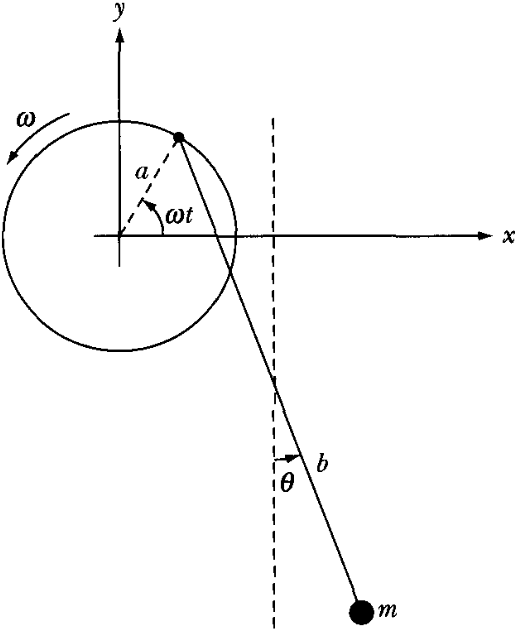
\includegraphics[width=0.75\textwidth]{marion_fig7_3.png}
		% 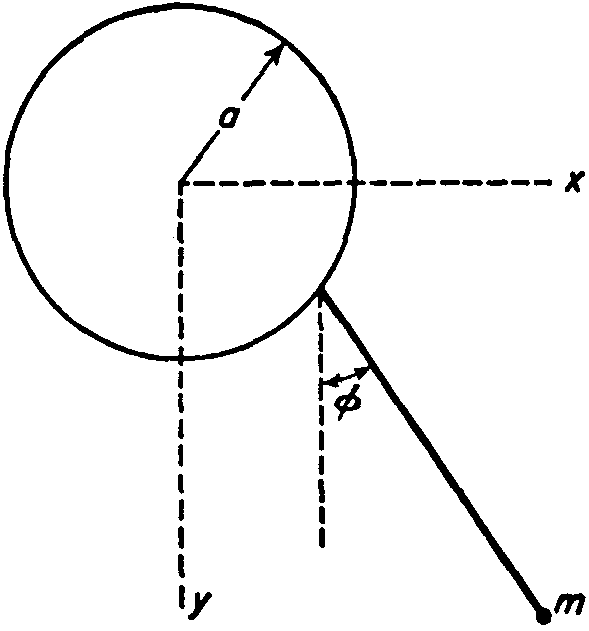
\includegraphics[width=0.75\textwidth]{landauS52_fig3.png}
	\end{minipage}



\item
	\begin{minipage}[t][4.5cm]{0.65\textwidth}
		(*) \textbf{Pesas acopladas rotando en torno a eje} [Landau \S5 ej. 4]\\

		La partícula con \(m_2\) se desplaza sobre un eje vertical, y todo el sistema gira con una velocidad angular constante \(\Omega\) en torno a ese eje.
		Dicha partícula está unida por barras de longitud \(a\) y masa despecible a otras dos de masa \(m_1\) que a su vez pendend de sendas barras idénticas del punto fijo \(A\) que describen un ángulo de apertura respecto al eje \(\theta\) que es variable.

			Calcule la energía cinética para cada una de las tres masas y exprese en la forma más compacta posible la del sistema en su conjunto.
	\end{minipage}
	\begin{minipage}[c][1cm][t]{0.35\textwidth}
		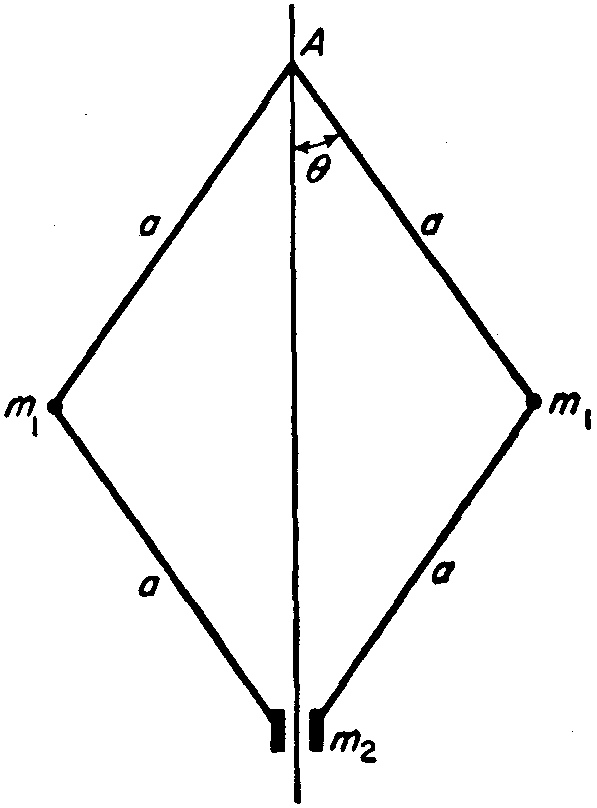
\includegraphics[width=0.75\textwidth]{landauS52_fig4.png}
	\end{minipage}



\end{enumerate}
\end{document}
